\paragraph{Question 1}
La complexité est de $O(m(n+m))=O(n^4)$ car~:
\begin{itemize}
\item La taille de la coupe augmente d'un sommet à chaque tour, donc
il nous faut $m$ étapes pour trouver la coupe maximum.
\item À chaque tour, on rajoute un également toutes les arêtes
incidentes au sommet rajouté.
\end{itemize}

\paragraph{Question 2}
Montrons que le taux d'approximation est de 2~:
\begin{proof}Soit $(Y_1,Y_2)$ la coupe approximatif. Supposons pour $\Gamma(x)$ l'ensemble des sommets voisins d'un sommet x~:

$\exists x \in Y_1 \text{ | } \Gamma(x) \cap Y_1 > \Gamma(x) \cap Y_2$

Dans un tel cas le déplacement du sommet x dans $Y_2$ augmenterai la valeur de la coupe, donc l'algorithme approché ne l'aurait jamais gardé dans $Y_1$. Notre supposition est donc absurde. Nous avions au contraire~:

$\forall x \in Y_1 \text{ | } \Gamma(x) \cap Y_1 \leq \Gamma(x) \cap Y_2$

Le même raisonnement tient pour les sommets de $Y_2$, donc globalement au pire la moité des arrêtes doivent traverser la coupe, soit \mbox{$(Y_1,Y_2) \geq \frac{|E|}{2}$}. Or même la coupe optimale est borné par $|E|$, donc $\frac{(Y_1,Y_2)}{(Y_1,Y_2)^*} \geq 2$, \emph{quod erat demonstrandum}.
\end{proof}

\paragraph{Question 3}

Nous pouvons construire l'instance ci-dessous pour laquelle la borne de
deux est atteinte. 
***************************************
***************************************
**************************************
TODO -- FINIR: énoncer la coupe optimale versus la coupe donné par l'algorithme, montrer que l'un est deux fois l'autre.

\begin{figure}[h!]
\centering
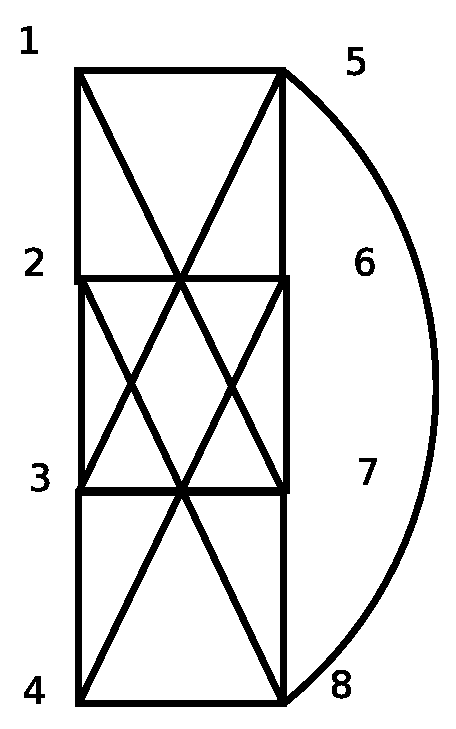
\includegraphics[height = 4cm]{../images/exo4.eps}
\caption{Instance où la borne de $2$ est atteinte, exercice 4}
\end{figure}
